\documentclass[a4paper,UKenglish,cleveref, autoref, thm-restate]{oasics-v2019}
%This is a template for producing OASIcs articles.
%See oasics-manual.pdf for further information.
%for A4 paper format use option "a4paper", for US-letter use option "letterpaper"
%for british hyphenation rules use option "UKenglish", for american hyphenation rules use option "USenglish"
%for section-numbered lemmas etc., use "numberwithinsect"
%for enabling cleveref support, use "cleveref"
%for enabling autoref support, use "autoref"
%for anonymousing the authors (e.g. for double-blind review), add "anonymous"
%for enabling thm-restate support, use "thm-restate"

%\graphicspath{{./graphics/}}%helpful if your graphic files are in another directory

\usepackage{tikz}
\usepackage{forest}
\usepackage{behaviortrees}
\usepackage{float}
\usepackage{caption}
\usepackage{subcaption}
\usetikzlibrary{shapes.geometric}
\usetikzlibrary{decorations.pathmorphing}

\usepackage{appendix}

\bibliographystyle{plainurl}% the mandatory bibstyle

\def\bht{BhTSL}
\title{\bht, Behavior Trees Specification and Processing} %TODO Please add

\titlerunning{\bht, Behavior Trees} %TODO optional, please use if title is longer than one line

\author{Miguel Oliveira}{Centro ALGORITMI, DI, Universidade do Minho, Portugal}{miguelmigpt@gmail.com}{}{}
\author{Pedro Mimoso Silva}{Centro ALGORITMI, DI, Universidade do Minho, Portugal}{pedro.miguel.mimoso@gmail.com}{}{}
\author{Pedro Moura}{Centro ALGORITMI, DI, Universidade do Minho, Portugal}{pedrorpmoura@gmail.com}{}{}
\author{José João Almeida}{Centro ALGORITMI, DI, Universidade do Minho, Portugal}{jj@di.uminho.pt}{}{}
\author{Pedro Rangel Henriques}{Centro ALGORITMI, DI, Universidade do Minho, Portugal}{prh@di.uminho.pt}{}{}


\authorrunning{M. Oliveira et al.} %TODO mandatory. First: Use abbreviated first/middle names. Second (only in severe cases): Use first author plus 'et al.'

\Copyright{Miguel Oliveira and Pedro M. Silva and Pedro Moura and José J. Almeida and Pedro R. Hemriques} %TODO mandatory, please use full first names. OASIcs license is "CC-BY";  http://creativecommons.org/licenses/by/3.0/

\ccsdesc[100]{\textcolor{red}{Replace ccsdesc macro with valid one}} %TODO mandatory: Please choose ACM 2012 classifications from https://dl.acm.org/ccs/ccs_flat.cfm

\keywords{Game development, Behavior trees (BT), NPC, DSL, Code generation} %TODO mandatory; please add comma-separated list of keywords

\acknowledgements{This work has been supported by FCT--Fundação para a Ciência e Tecnologia
within the R\&D Units Project Scope: UIDB/00319/2020.}%optional

%\nolinenumbers %uncomment to disable line numbering

%\hideOASIcs  %uncomment to remove references to OASIcs series (logo, DOI, ...), e.g. when preparing a pre-final version to be uploaded to arXiv or another public repository

%Editor-only macros:: begin (do not touch as author)%%%%%%%%%%%%%%%%%%%%%%%%%%%%%%%%%%
\EventEditors{Alberto Simões and Ricardo Queirós and Pedro Rangel Henriques}
\EventNoEds{3}
\EventLongTitle{9.th Symposium on Languages, Applications and Technologies (SLATE 2020)}
\EventShortTitle{SLATE 2020}
\EventAcronym{SLATe} 
\EventYear{2020}
\EventDate{July 13--14, 2020}
\EventLocation{IPCA -- Barcelos, Portugal}
\EventLogo{}
\SeriesVolume{}
\ArticleNo{}
%%%%%%%%%%%%%%%%%%%%%%%%%%%%%%%%%%%%%%%%%%%%%%%%%%%%%%

\begin{document}

\maketitle

%TODO mandatory: add short abstract of the document
\begin{abstract}
In the context of game development, there is always the need for describing behaviors for various entities, 
whether NPCs or even the world itself.
That need requires a formalism to describe properly such behaviors.
%
As the gaming industry has been growing, many approaches were proposed.
First, finite state machines were used and evolved to hierarchical state machines.
As that formalism was not enough, a more powerful concept appeared.
Instead of using states for describing behaviors, people started to use tasks.
This concept was incorporated in behavior trees.
%
This paper focuses in the specification and processing of Behavior Trees.
A DSL designed for that purpose will be introduced.
It will also be discussed a generator that produces \LaTeX\ diagrams to document the trees, 
and a Python module to implement the behavior described.
Additionally, a simulator will be presented.
These achievements will be illustrated using a concrete game as a case study.
\end{abstract}


\section{Introduction}
\label{sec:introduction}

At some point in the video-game history, NPCs (Non-Playable Characters) were introduced.
With them came the need to describe behaviors.
And with these behaviors came the need of the existence of a formalism so that they can be properly specified.

As time passed by, various approaches were proposed and used, like finite and hierarchical state machines.
These are state-based behaviors, that is, the behaviors are described through states.
Altough this is a clear and simplistic way to represent and visualize small behaviors, it becomes unsustainable when dealing with bigger and more complex behaviors.
Some time later, a new and more powerful concept was introduced: using tasks instead of states to describe behaviors.
This concept is incorporated in what we call behavior trees.

Behavior Trees (\texttt{BT} for short) were first used in the videogame industry in the development of the game \textit{Halo 2}, released in 2004 \cite{Cuadrado2018}.
The idea is that people create a complex behavior by only programming actions (or tasks) and then design a tree structure whose leaf nodes are actions and the inner nodes determine the NPC's decision making.
Not only these provide an easy and intuitive way of visualizing and designing behaviors, they also provide a good way to work with scalability through modularity, solving the biggest issue from state-based design.
Since then, multiple gaming companies adopted this concept and, in recent years, behavior trees are also being used in different areas like Artificial Inteligence and Robotics.

% Motivação
In this context, we felt that it could be useful to have a DSL to specify BTs independently of application area and the programming language chosen for the implementation.
The language must be compact and easy to use but it should be expressive enough to be applied to real situations.
In that sense a new kind of node was included, as will be described.

% Design goals
This paper will introduce the DSL designed and the compiler implemented to translate it to a programming language, in this case Python.
Additionally, the compiler also generates \LaTeX\ diagrams to produce graphical documentation for each BT specified.

A small example will be described in our language as a case study to illustrate all the achievements attained.

% Estrutura do artigo
The paper is organized as follow: Concepts and State of the Art frameworks are presented in Section \ref{sec:concepts}.
Architecture and language specification are proposed in Section \ref{sec:arc-spec}.
Compiler development is discussed in Section \ref{sec:tool_development}.
An illustrative example is presented in Section \ref{sec:example}, 
before concluding the paper in Section \ref{sec:conclusion}.
The paper also includes two appendices, one that contains the tokens table,
 and another to show the complete specification of \texttt{TGame} used as an example.

\section{Concepts}
\label{sec:concepts}

This section will be built based on references \cite{ColOgr2018,Simpson2014,MilFunge2009}.

Formally, a BT is a tree whose internal nodes are called control flow nodes and leafs are called execution nodes.

% descrever a execução
A behavior tree executes by peridiocally sending ticks to its children, in order to traverse the entire tree.
Each node, upon a tick call, returns one of the following three states to its parent: \texttt{SUCCESS} if the node was executed with success; \texttt{FAILURE} if the execution failed; or \texttt{RUNNING} if it could not finish the execution by the end of the tick.
In the last case, the next tick will traverse the tree until it reaches the running execution node, and will try again to run it.

\subsection{Control Flow Nodes}
Control flow nodes are structural nodes, that is, they do not have any impact in the state of the system. They only control the way the subsequent tree is traversed.
In the classical formulation, there are 4 types of control flow nodes: \textbf{Sequence}, \textbf{Selector}, \textbf{Parallel} and \textbf{Decorator}.
Even if not standard we use decorators as control flow nodes, according to \cite{ColOgr2018}.
A sequence node (figure \ref{fig:sequence}) visits its children in order, starting with the first, and advancing for the next one if the previous succeeded.
Returns:
\begin{itemize}
    \item \texttt{SUCCESS} - if all children succeed;
    \item \texttt{FAILURE} - if a child fails;
    \item \texttt{RUNNING} - if a child returns \texttt{RUNNING}.
\end{itemize}


Like the sequence, the selector node (figure \ref{fig:selector}) also visits its children in order, but it only advances if the child that is being executed returns \texttt{FAILURE}.
Returns:
\begin{itemize}
    \item \texttt{SUCCESS} - if a child succeeds;
    \item \texttt{FAILURE} - if all children fails;
    \item \texttt{RUNNING} - if a child returns \texttt{RUNNING}.
\end{itemize}


A parallel node (figure \ref{fig:parallel}), as the name implies, visits its children in parallel.
Additionally, it has a parameter $M$ that acts as a success rate.
For $N$ children and $M \leq N$, it returns:
\begin{itemize}
    \item \texttt{SUCCESS} - if $M$ children succeed;
    \item \texttt{FAILURE} - if $N - M + 1$ children fail;
    \item \texttt{RUNNING} - otherwise.
\end{itemize}



A decorator (figure \ref{fig:decorator}) is a special node that has an only one child, and uses a policy (set of rules) to manipulate the return status of its child, or the way it ticks it.
Some examples of decorator nodes are:
\begin{enumerate}
    \item \textbf{Inverter} - inverts the \texttt{SUCCESS}/\texttt{FAILURE} return status of the child;
    \item \textbf{Max-$N$-Times} - the child can only fail $N$ times.
    After that it only returns \texttt{FAILURE} without ticking the child.
\end{enumerate}

\subsection{Execution Nodes}
Execution nodes are the simplest, yet the most powerful. They are the ones that have access to the state of the system, and can update it.
There are two types of execution nodes: \textbf{Action} and \textbf{Condition}.


Upon the execution of a tick, an action node (figure \ref{fig:action}) runs a chunk of code that can return either \texttt{SUCCESS}, \texttt{FAILURE} or \texttt{RUNNING}


The condition node (figure \ref{fig:condition}) verifies a proposition, returning \texttt{SUCCESS}/\texttt{FAILURE} if the proposition is/is not valid.
This node never returns \texttt{RUNNING}.


\begin{figure}[h]
    \begin{subfigure}{.5\textwidth}
        \centering
        \captionsetup{justification=centering}
        \begin{behavior}
            [\sequence
                [\action{Child 1}]
                [{\textbf{. . .}}, inner sep=10pt]
                [\action{Child N}]
            ]
        \end{behavior}
        \caption{Sequence node.}
        \label{fig:sequence}
    \end{subfigure}%
    \begin{subfigure}{.5\textwidth}
        \centering
        \captionsetup{justification=centering}
        \begin{behavior}
            [\decorator{$\delta$},
                [\action{Child}]
            ]
        \end{behavior}
        \caption{\textit{Decorator} with policy $\delta$.}
        \label{fig:decorator}
    \end{subfigure}\\
    \begin{subfigure}{.5\textwidth}
        \centering
        \captionsetup{justification=centering}
        \begin{behavior}
            [\selector
                [\action{Child 1}]
                [{\textbf{. . .}}, inner sep=10pt]
                [\action{Child N}]
            ]
        \end{behavior}
        \caption{Selector node.}
        \label{fig:selector}
    \end{subfigure}%
    \begin{subfigure}{.5\textwidth}
        \centering
        \captionsetup{justification=centering}
        \begin{behavior}
            [\action{Action}]
        \end{behavior}
        \caption{\textit{Action} node.}
        \label{fig:action}
    \end{subfigure}\\
    \begin{subfigure}{.5\textwidth}
        \centering
        \captionsetup{justification=centering}
        \begin{behavior}
            [\parallel{M}
                [\action{Child 1}]
                [{\textbf{. . .}}, inner sep=10pt]
                [\action{Child N}]
            ]
        \end{behavior}
        \caption{Parallel node.}
        \label{fig:parallel}
    \end{subfigure}%
    \begin{subfigure}{.5\textwidth}
        \centering
        \captionsetup{justification=centering}
        \begin{behavior}
            [\condition{Condition}]
        \end{behavior}
        \caption{\textit{Condition} node.}
        \label{fig:condition}
    \end{subfigure}

    \caption{BT Nodes structure.}
\end{figure}


% Memory
\subsection{Control Flow Nodes with memory}
Sometimes, when a node returns \texttt{RUNNING}, we want it to remember which nodes he already executed, so that the next tick does not execute them again.
We call this nodes with memory.
And they are represented by adding a $\_^*$ to the symbols mentioned previously.
This is only sintatic sugar because we can also represent these nodes with a non-memory BT, but that will not be discussed here.

Please note that, while we avoid the re-execution of nodes with this type of node, we also lose the reactivity that this re-execution provides.

\subsection{State of The Art}
\label{subsec:state-of-the-art}
In the gaming industry there is some interesting projects that use tools based on Behavior trees as the main focus to describe NPCs behaviors.
Unreal Engine \cite{UnrealEngine} and Unity\footnote{\raggedright\url{https://unity.com}} are two examples of major game engines that use them.
In their case, instead of a language, they offer a graphical user interface (GUI) to specify the BTs, through a drag and drop tactic.
Upon the creation of an execution node, the programmer needs to specify the action or condition that will be executed.
The nodes mentioned before are all implemented in these engines, along with some extensions.
All the nodes that were mentioned before are implemented in both of these engines, along with some extensions.

In addition to game engines, there are also frameworks like Java Behavior Trees\footnote{\url{https://github.com/gaia-ucm/jbt}} for Java and Owyl\footnote{\url{https://github.com/eykd/owyl}} for Python that implement BTs.
In this case, they work as a normal library.

\section{Architecture and Specification}
\label{sec:arc-spec}
In this section, it will be explained the general architecture of our system to process BTs, 
that is depicted in Figure \ref{fig:architecture}. 
After introducing its modules, one subsection is devoted to the \bht\ domain specific language design.
\begin{figure}[h]
    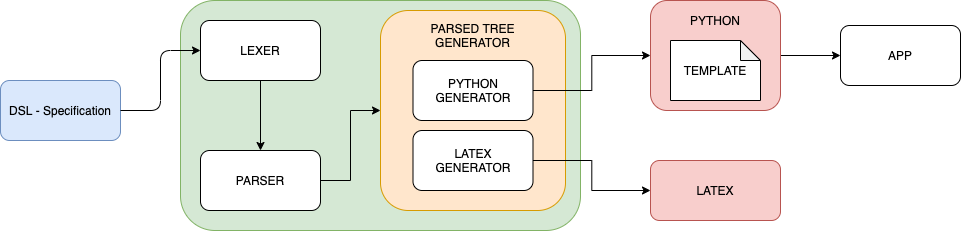
\includegraphics[width=\columnwidth]{architecture.png}
    \caption{System Architecture.}
    \label{fig:architecture}
\end{figure}

The input for our system, \texttt{DSL - Specification}, is a text file describing the behavior which 
should follow the language syntax.
The compiler, which is represented as the green rounded rectangle in the diagram of Figure~\ref{fig:architecture}, 
is composed of the following modules: a \texttt{Lexer}, a \texttt{Parser} and a \texttt{Code Generator}.\\
This generator has two sub-generators.
The \texttt{Latex Generator}, that is responsible for the generation of the \LaTeX\ code to draw
the tree diagram representing the behavior specified.
And the \texttt{Python Generator}, that produces the fragment of Python code that implements
the desired  behavior according to a template predefined by us in the context of this project;
that code fragment can be later imported by  any Python application that aims to.

\subsection{\bht}

Before we start describing the DSL, we will introduce a new node, called \textbf{Probability Selector} 
(Figure \ref{fig:prob_selector} depicts that concept), that  provides us with a relevant extension to the standard
formalism for a more powerful  behavior specification.
This extension improves the expressiveness of \bht\ language.

A probability selector node is like a normal selector node, but instead of visiting its children from left to right, 
it visits them randomly, taking into account that each child has a probability, defined by the user, 
of being chosen first.

\begin{figure}[H]
    \centering
    \begin{behavior}
        [\probselector
            [\probnodeaction{$P_1$}{Child 1}],
            [\probnodeaction{$P_2$}{Child 2}],
            [{\textbf{. . .}}, inner sep=10pt],
            [\probnodeaction{$P_N$}{Child N}]
        ]
    \end{behavior}
    \caption{Probability Selector node.}
    \label{fig:prob_selector}
\end{figure}

\paragraph*{Example}{
    Now that all nodes have been introduced, let us see an example of a specific behavior.

    Suppose that in some game, called \texttt{TGame}, 
    it is intended  to have a \emph{guard that patrols a house}.
    The guard has the following behavior: while he is patrolling, if he sees the player, activates an alarm and then, 
    depending on the level of courage he has, decides (based on probabilities) whether he runs away or fights the player.
    In case of running away, he constantly checks if he still sees the player, returning to patrolling in case he does not. 
    If he still sees it, he keeps running.
    The same thing happens when he chooses to fight the player, only this time he checks if the player is already dead 
    or not.

    In Figure \ref{fig:example}, we can see a possible tree specification for this behavior.

    \begin{figure}[h]
        \centering
        \begin{behavior}
            [\rootnode
                [\selector
                    [\memorysequence
                        [\condition{sees player}]
                        [\action{activate alarm}]
                        [\memoryprobselector
                            [\probnodesequence{$e1$}
                                [\inverter
                                    [\condition{player dead}]
                                ]
                                [\action{fight player}]
                            ]
                            [\probnodesequence{$e2$}
                                [\condition{sees player}]
                                [\action{run}]
                            ]
                        ]
                    ]
                    [\action{patrol}]
                ]
            ]
        \end{behavior}
        \caption{Example: \texttt{TGame} behavior tree diagram automatically generated by our tool }
        \label{fig:example}
    \end{figure}
}

\subsubsection{Syntax}
In our language, each specification represents one and only one behavior.
An  input file, containing the behavior specification text, is divided into 3 components:
\begin{itemize}
    \item \textit{Behavior} - main behavior tree;
    \item \textit{Definitions} (optional) - node definitions that can be referenced in other nodes or in the main BT;
    \item \textit{Code} - Python block that contains the code fragments described the execution nodes, and other code that the programmer wishes to add.
\end{itemize}

To illustrate our idea about the DSL we plan to design (formally defined by a grammar in section~\ref{sec:tool_development}),
we present below an example of a specification written in the intended language.
\begin{lstlisting}
behavior : [
    sequence : [
        condition : $cond1,
        condition : $cond2
        memory selector : [
            parallel : $par1,
            prob_selector : $prob1
        ]
    ]
]

parallel par1 : 10 [
    action : $action1,
    action : $action2
]

prob_selector prob1 : [
    $e1 -> decoraror : INVERTER [
        action : $action1
    ],
    $e2 -> action : $action2
]

%%

def action1(entity):
    pass

def action2(entity):
    pass

def cond1(entity):
    pass

def cond2(entity):
    pass

def e1(entity):
    pass

def e2(entity):
    pass
\end{lstlisting}

\section{Tool development}
\label{sec:tool_development}
In the next subsection the implementation of the \bht\ processor will be detailed, as well as the language 
specification will be presented.

\subsection{Lexical analysis}
The first step in the development of a compiler is the lexical analysis, that converts a char sequence 
into a token sequence.
The tokens table can be seen in Ãppendix\label{apx:TokTab}.

\subsection{Syntatic analysis}
Syntatic analysis, or parsing, it the process of analyzing a string of symbols conforming the rules of a grammar. \\
Below  we list the context free grammar that formally specifies \bht\ syntax:
\begin{lstlisting}
    root : behavior CODE
         | behavior definitions CODE
         | definition behavior CODE

    behavior : BEHAVIOR ':' '[' node ']'

    node : SEQUENCE ':' '[' nodes ']'
         | SEQUENCE ':' VAR
         | MEMORY SEQUENCE ':' '[' nodes ']'
         | MEMORY SEQUENCE ':' VAR
         | SELECTOR ':' '[' nodes ']'
         | SELECTOR ':' VAR
         | MEMORY SELECTOR ':' '[' nodes ']'
         | MEMORY SELECTOR ':' VAR
         | PROBSELECTOR ':' '[' prob_nodes ']'
         | PROBSELECTOR ':' VAR
         | MEMORY PROBSELECTOR ':' '[' prob_nodes ']'
         | MEMORY PROBSELECTOR ':' VAR
         | PARALLEL ':' INT '[' nodes ']'
         | PARALLEL ':' VAR
         | DECORATOR ':' INVERTER '[' node ']'
         | DECORATOR ':' VAR
         | CONDITION ':' VAR
         | ACTION ':' VAR

    nodes : nodes ',' node
          | node

    prob_nodes : prob_nodes ',' prob_node
               | prob_node

    prob_node : VAR RIGHTARROW node

    definitions : definitions definition
               | definition

    definition : SEQUENCE NODENAME ':' '[' nodes ']'
        | SELECTOR NODENAME ':' '[' nodes ']'
        | PROBSELECTOR NODENAME ':' '[' prob_nodes ']'
        | PARALLEL NODENAME ':' INT '[' nodes ']'
        | DECORATOR NODENAME ':' INVERTER '[' node ']'
\end{lstlisting}

\subsection{Semantic analysis}
As usual, from a static semantics perspective, the compiler will check the source text 
for non-declared variables and variable redeclaration.\\
A variable can only be accessed if it is declared, either in the \textit{definitions} section 
(if it represents a control flow node), or in the \textit{code} section (execution node).
Additionally, a variable can only be declared one time, to avoid ambiguity in the memory access by the processor.


%% Dynamic and Static Semantics

\subsection{Code generator}
The compiler can generate two different outputs: 
a \LaTeX\ file, that contains the \LaTeX\ commands to draw a diagram for the BT specified; 
and a Python file, that contains the functions that implement the specified behavior.


The output Python file is built using a \textbf{Template} file which contains markers that the \textbf{Code Generator} will fill with the processed data. 
This file also contains the class \textbf{Simulator} which is capable of executing the processed BT.

Due to the lack of time available, we've only been able to generate Python code, but we hope to be able to compile into different languages in the future.

%% Cross-compiling 

%% Mention templates

\subsection{BT Simulator}
In order to test the Python code generated and to help the BT specifier to debug the behavior he is willing
to describe, we also developed an interpreter that imports the Python behavior file and simulates its
execution.
This additional tool proved to be useful. 

\subsection{Implementation}


The project was developed using \texttt{Python}.
We chose this language due to our previous experience with it, but also due to its simplicity, flexibility and its cutting edge technology; it is also relevant to be a reflective language. 

To automatically generate the compiler from the tokens and grammar specifications, 
we used the \texttt{PLY (Python Lex-Yacc)}\footnote{\url{https://www.dabeaz.com/ply/}} library, which is an implementation of the \texttt{lex} and \texttt{yacc} lexer and parser generator tools for Python.
We chose to use PLY because we had prior experience with Lex-Yacc which enabled us to save time to implement the project.
Moreover, we realized that the specification is lighter than an equivalent using attribute grammars and because the code produced by those generators is really efficient.

To implement the \textbf{Code Generator} module, we resorted to the well-known tree-traversal approach, that upon visiting every node of the parsed tree, produces the corresponding output.
For that purpose, some standard libraries were used.

Additionally, we created a \LaTeX\ library, \texttt{behaviortrees.sty}, to draw the trees specified. 
This library is used in the \LaTeX\ generator.

\section{Case Study}
In order to test our tool, we designed a simple game that consists of an entity finding and grabbing a ball in a generated map.
This entity has a range of vision that it is used to search the ball.
When the entity finds it, it approaches the ball and, if it is within reach, grabs it.

The following code is an example of a specification for this behavior in our DSL, and Figure \ref{fig:case_study_bt} depicts the behavior tree automatically generated by our tool.
\begin{lstlisting}
behavior : [
    selector : [
        memory sequence : $seq1,
        action : $search_ball
    ]
]

sequence seq1 : [
    condition : $ball_found,
    selector : [
        sequence : [
            condition : $ball_within_reach,
            action : $grab_ball
        ],
        action : $approach_ball
    ]
]


%%

def ball_found(player):
    return player.ball_found


def ball_within_reach(player):
    return player.ball_within_reach


def grab_ball(player):
    player.grab_ball()
    return SUCCESS


def approach_ball(player):
    player.approach_ball()
    return RUNNING


def search_ball(player):
    player.search_ball()
    return RUNNING
\end{lstlisting}

\begin{figure}
    \centering
    \begin{behavior}
        [\rootnode
            [\selector
                [\memorysequence
                    [\condition{ball found}]
                    [\selector
                        [\sequence
                            [\condition{ball within reach}]
                            [\action{grab ball}]
                        ]
                        [\action{approach ball}]
                    ]
                ]
                [\action{search ball}]
            ]
        ]
    \end{behavior}
    \caption{Behavior Tree generated from the case study.}
    \label{fig:case_study_bt}
\end{figure}

Now that we have the specification, we can generate the \texttt{Python} file to use in our code.
Suppose that the generated file's name is \texttt{behavior.py}, we can import it by writing \texttt{import behavior}.
With this, we can make use of the \textbf{Simulator} class to execute the behavior.

Next is a code example of how we can use this class to run the behavior.

\begin{lstlisting}
game = Game()
game.setup()
S = behavior.Simulator(game.player1)

game.render(screen)

while True:
    
    game.process_events()

    S.tick()
    game.update(clock, 2)
    game.render(screen)
\end{lstlisting}

According to the specification, our entity can perform 3 different actions: search for the ball, approach the ball, and grab the ball.

Searching for the ball occurs in an initial moment, in which the entity does not know yet where the ball is.
Figure \ref{fig:searching} depicts an example of that moment, where the entity is the blue square and the ball is the red square.
\begin{figure}
    \centering
    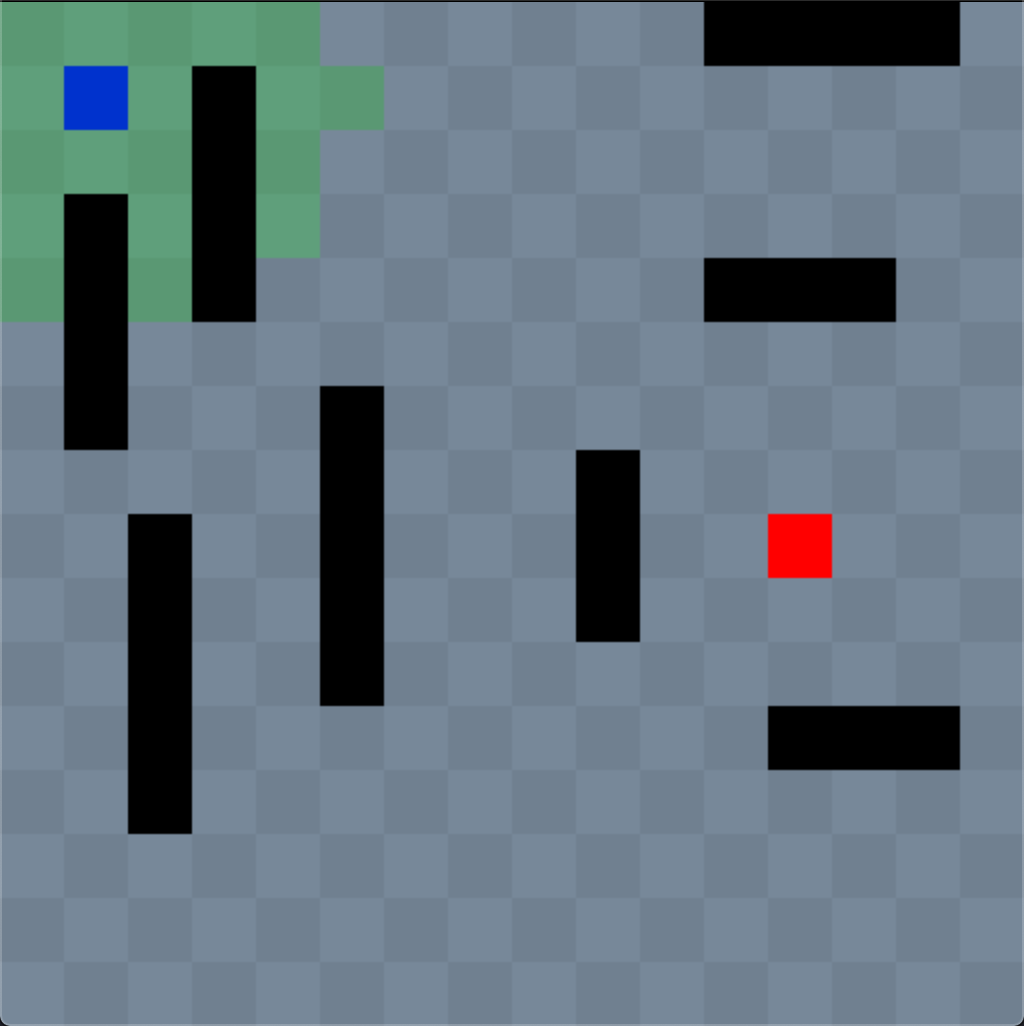
\includegraphics[width=6cm]{Searching.png}
    \caption{Searching for the ball.}
    \label{fig:searching}
\end{figure}

Until it finds the ball, the entity roams freely through the map.

When it finds it, unless it is within arms reach, the entity will approach it.
Figure \ref{fig:approaching} depicts the moment when the entity found the ball.
\begin{figure}
    \centering
    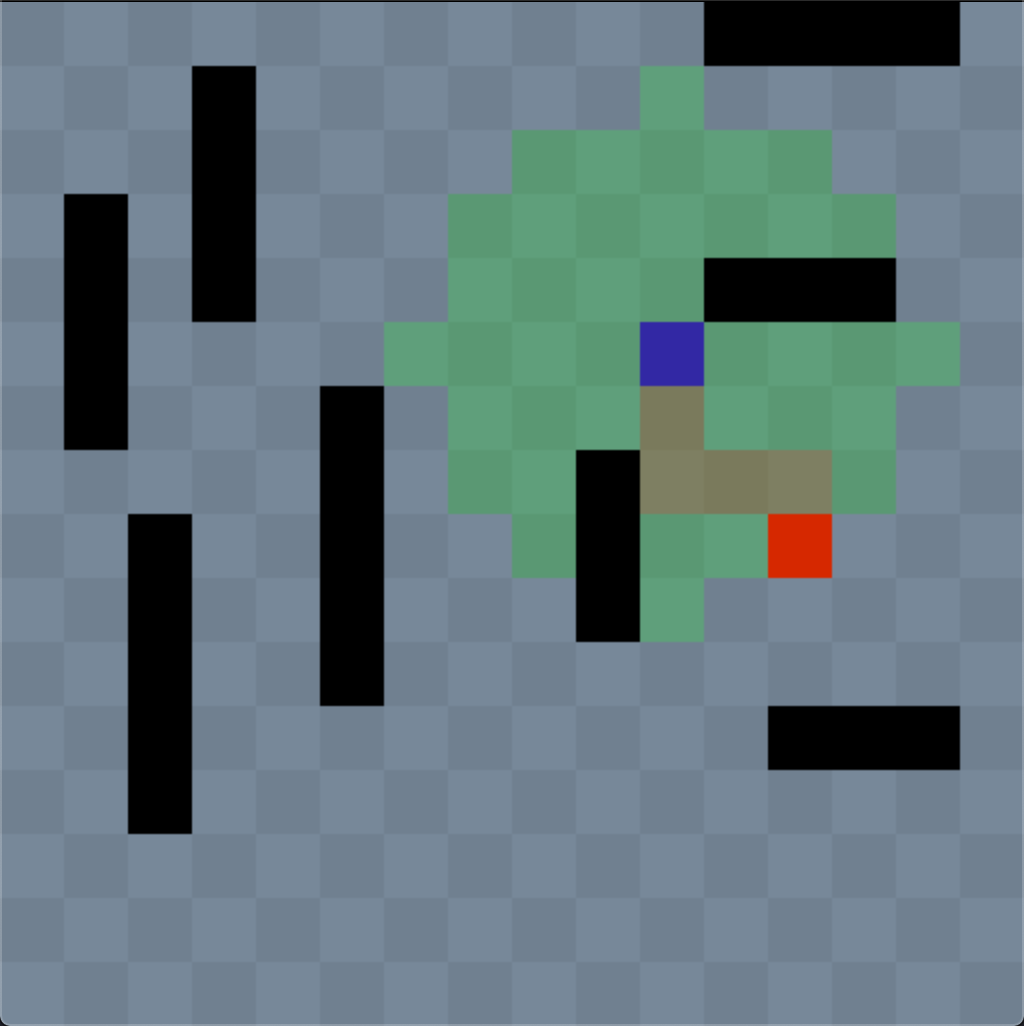
\includegraphics[width=6cm]{Approaching.png}
    \caption{Approaching the ball.}
    \label{fig:approaching}
\end{figure}

Lastly, when the ball is within reach, the entity grabs it, as it is shown in Figure \ref{fig:grabbing}.

\begin{figure}
    \centering
    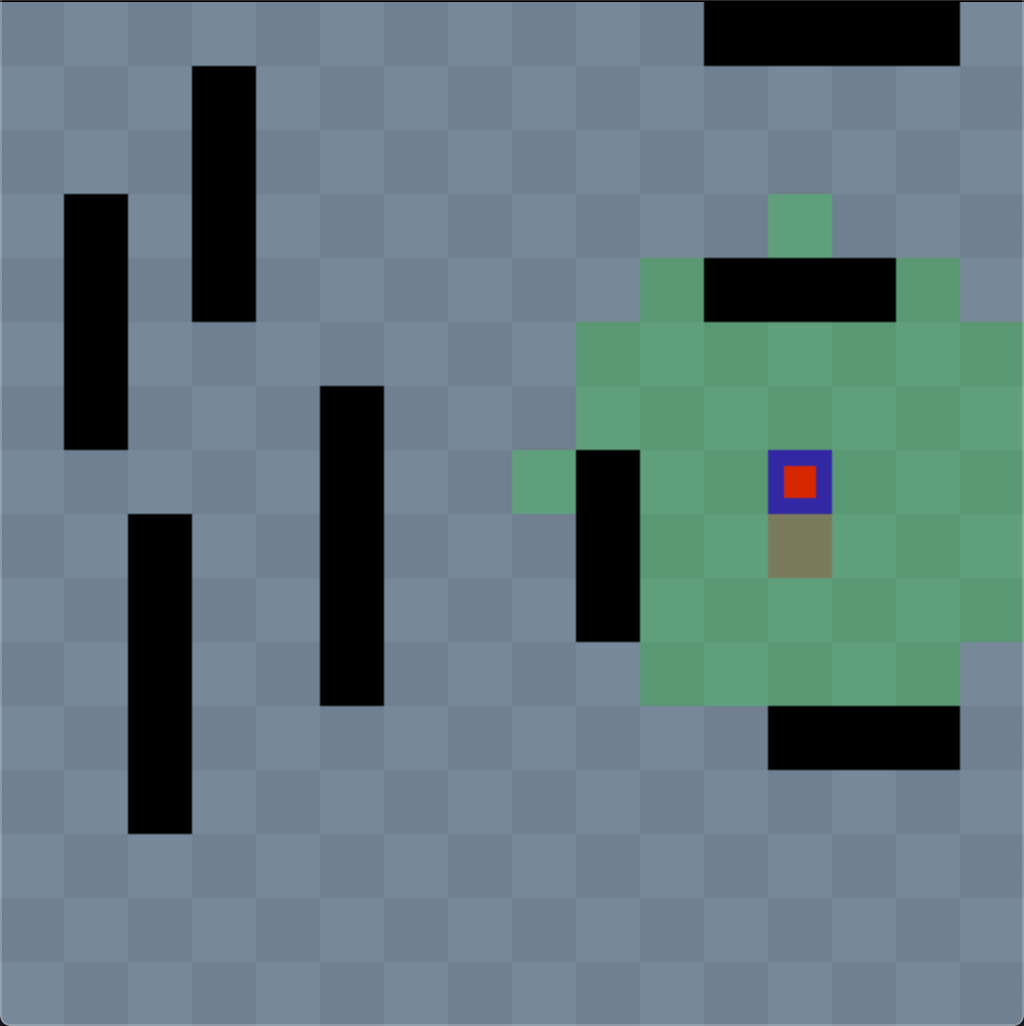
\includegraphics[width=6cm]{Grabbing.png}
    \caption{Grabbing the ball.}
    \label{fig:grabbing}
\end{figure}


\section{Conclusion}
\label{sec:conclusion}

As games industry is growing significantly every day, the need for a formal way to describe behaviors  
is also increasing requiring more and more expressiveness keeping it easy to learn, to use and to understand.
After some initial attempts not powerful enough, a new approach called Behavior Trees (BT) appeared.
This paper describes a project in which we are working on, aimed at designing a DSL to write BT
and developing the respective compiler to generator Python functions to be incorporated in final Python
programs created to implement games or other kind of applications.

Along the paper the DSL designed, called \bht, was introduced by example and specified by a context 
free grammar. 
The architecture of the \bht\ processor was depicted and discussed, and the development of the compiler that produces the
Python code library  was described.
In that context an example of a game  specification was presented and the \LaTeX\ fragment that is
 generated to draw the BT was shown.
 
Although not detailed or exemplified, the simulator developed to help on debugging the BT specified in
\bht\ language was mentioned along the paper. 

\subsection{Future Work}
As future work we intend to implement the generation of code for other programming languages, such as Java and C++ so that it can be widely used by the game development community.
This should be a fairly standard procedure due to our usage of templates on the \textbf{Code Generation} stage of our program.


\bibliography{behavior_trees}

%\newpage
\begin{appendices}

\section{Tokens Table}
\label{apx:TokTab}
The following table displays the full set of  tokens of \bht\ language
defined in terms of regular expressions (REs)  as utilized in our compiler.
\begin{table}[H]
    \centering
    \begin{tabular}{ | p {5cm} | p {5cm} | }
        \hline
            \multicolumn{2}{ |c| }{\textit{\textbf{Tokens}}} \\
        \hline
            \multicolumn{1}{ |c| }{\textbf{Name}} & \multicolumn{1}{ |c| }{\textbf{Value}} \\
        \hline
        \hline
            literals         & \texttt{({[]}),:\%}           \\ \hline
            RIGHTARROW       & \texttt{->}                   \\ \hline
            BEHAVIOR         & \texttt{\textbackslash bbehavior\textbackslash b}     \\ \hline
            SEQUENCE         & \texttt{\textbackslash bsequence\textbackslash b}     \\ \hline
            SELECTOR         & \texttt{\textbackslash bselector\textbackslash b}     \\ \hline
            PROBSELECTOR     & \texttt{\textbackslash bprobselector\textbackslash b} \\ \hline
            PARALLEL         & \texttt{\textbackslash bparallel\textbackslash b}     \\ \hline
            DECORATOR        & \texttt{\textbackslash bdecorator\textbackslash b}    \\ \hline
            CONDITION        & \texttt{\textbackslash bcondition\textbackslash b}    \\ \hline
            ACTION           & \texttt{\textbackslash baction\textbackslash b}       \\ \hline
            INVERTER         & \texttt{\textbackslash bINVERTER\textbackslash b}     \\ \hline
            MEMORY           & \texttt{\textbackslash bmemory\textbackslash b}       \\ \hline
            INT              & \texttt{\textbackslash d+}                            \\ \hline
            VAR              & \texttt{\$\textbackslash w+}                          \\ \hline
            NODENAME         & \texttt{\textbackslash b\textbackslash w+\textbackslash b}   \\ \hline
            CODE             & \texttt{\%\%(.|\textbackslash n)+} \\
        \hline
    \end{tabular}\\
    \caption{\bht\ Tokens Table for Lexical Analysis.}
    \label{tab:tokens}
\end{table}

%\section{Example Specification}
%\label{appendix:example_specification}
%This appendix lists the \texttt{TGame} full specification that is an example
%of a game formal description in \bht.
%\begin{lstlisting}
%behavior : [
%    selector : [
%        memory sequence : [
%            condition : $sees_player,
%            action : $activate_alarm,
%            memory prob_selector : [
%                $e1 -> sequence : [
%                    decorator : INVERTER [
%                        condition : $player_dead
%                    ],
%                    action : $fight_player
%                ],
%                $e2 -> sequence : [
%                    condition : $sees_player,
%                    action : $run
%                ]
%            ]
%        ],
%        action : $patrol
%    ]
%]
%
%%%
%def sees_player(patroller):
%    from math import sqrt
%    player_x = patroller['player']['x']
%    player_y = patroller['player']['y']
%
%    patroller_x = patroller['x']
%    patroller_y = patroller['y']
%
%    if sqrt(patroller_x ** 2 - player_x** 2 +
%     patroller_y**2 - player_y**2) <= patroller['vision_radius']:
%        return SUCCESS
%
%    return FAILURE
%
%
%def activate_alarm(patroller):
%    print("ALARM ACTIVATED!!")
%    patroller['alarm_activated'] = True
%    return SUCCESS
%
%
%def player_dead(patroller):
%    if patroller['player']['hp'] == 0:
%        return SUCCESS
%    return FAILURE
%
%
%def fight_player(patroller):
%    patroller['player']['hp'] -= 10
%    return RUNNING
%
%
%def run(patroller):
%    patroller['x'] = patroller['x'] - 10
%    patroller['y'] = patroller['y'] - 10
%
%    print("Running away from player!")
%    return RUNNING
%
%
%def patrol(patroller):
%    patroller['x'] = patroller['x'] + 10
%    patroller['y'] = patroller['y'] + 10
%    return RUNNING
%
%
%def e1(patroller):
%    return patroller['guts'] / 10
%
%def e2(patroller):
%    return 1 - patroller['guts'] / 10
%\end{lstlisting}


\end{appendices}


\end{document}
